%% --------------------------------------------------------------
%% 
%% Copyright (C) 2001
%% Michael McNeil Forbes
%% mforbes@alum.mit.edu
%% 
%% This file may be distributed and/or modified under the
%% conditions of the LaTeX Project Public License, either version 1.2
%% of this license or (at your option) any later version.
%% The latest version of this license is in
%%    http://www.latex-project.org/lppl.txt
%% and version 1.2 or later is part of all distributions of LaTeX
%% version 1999/12/01 or later.
%% 
%% This program is distributed in the hope that it will be useful,
%% but WITHOUT ANY WARRANTY; without even the implied warranty of
%% MERCHANTABILITY or FITNESS FOR A PARTICULAR PURPOSE.  See the
%% LaTeX Project Public License for more details.
%% 
%% This program consists of the files ubcthesis.dtx, ubcthesis.ins, and
%% the sample figures fig.eps and fig.fig.
%% 
%% This file may be modified and used as a base for your thesis without
%% including the licence agreement as long as the content (i.e. textual
%% body) of the file is completely rewritten. You must, however, change
%% the name of the file.
%% 
%% This file may only be distributed together with a copy of this
%% program. You may, however, distribute this program without generated
%% files such as this one.
%% 

% This Sample thesis requires \LaTeX2e
\NeedsTeXFormat{LaTeX2e}[1995/12/01]
\ProvidesFile{ubcsample.tex}[2012/04/07 v1.70 ^^J
 University of British Columbia Sample Thesis]
% This is the \documentclass[]{} command.  The manditory argument
% specifies the "flavour" of thesis (ubcthesis for UBC).  The
% optional arguments (in []) specify options that affect how the
% thesis is displayed.  Please see the ubcthesis documentation for
% details about the options.
\documentclass[msc,oneside]{ubcthesis}
%
%************************************************
% Optional packages.
%
% The use of these packages is optional, but they provide various
% tools for more flexible formating.  The sample thesis uses these,
% but if you remove the example code, you should be able to exclude
% these packages.  Only standard packages have been described here;
% they should be installed with any complete LaTeX instalation, but
% if not, you can find them at the Comprehensive TeX Archive Network
% (CTAN): http://www.ctan.org/
%

%******** afterpage ***************************
% This package allows you to issue commands at the end of the current
% page.  A good use for this is to use the command
% \afterpage{\clearpage} right after a figure.  This will cause the
% figure to be inserted on the page following the current one (or on
% the current page if it will fit) but will not break the page in the
% middle.
\usepackage{afterpage}

%******** float *********************************
% This package allows you to customize the style of
% "floats"---floating objects such as figures and tables.  In
% addition, it allows you to define additional floating objects which
% may be included in a list similar to that produces by \listoftables
% and \listoffigures.  Common uses include introducing floats for
% programs and other code bits in Compute Science and Chemical Schema.
\usepackage{float}

%******** tocloft *******************************
% This package allows you to customize and define custom lists such
% as a list of programs or Chemical Scheme.  Note: if you use the
% subfigure package, you must specify that you do as an option here.
% The title option uses the default formatting.  We do not use this
% here as the default formatting is acceptable.  Use the float
% package instead unless you need the extra formatting control
% provided by tocloft.
%\usepackage[subfigure, titles]{tocloft}

%******** alltt *********************************
% The alltt package allows you to include files and have them
% formatted in a verbatim fashion.  This is useful for including
% source code from an additional file.
%\usepackage{alltt}

%******** listings ******************************
% The listings package may be used to include chunks of source code
% and has facilities for pretty-printing many languages.
%\usepackage{listings}

%******** longtable *****************************
% The longtable package allows you to define tables that span
% multiple pages.
\usepackage{longtable}

%******** graphics and graphicx *****************
% This allows you to include encapsulated postscript files.  If you
% don't have this, comment the \includegraphics{} line following the
% comment "%includegraphics" later in this file.
\usepackage{graphicx}

%******** subfigure *****************************
% The subfigure package allows you to include multiple figures and
% captions within a single figure environment.
%\usepackage{subfigure}

%******** here **********************************
% The here package gives you more control over the placement of
% figures and tables.  In particular, you can specify the placement
% "H" which means "Put the figure here" rather than [h] which means
% "I would suggest that you put the figure here if you think it looks
% good."
%\usepackage{here}

%******** pdflscape ********************************
% This allows you to include landscape layout pages by using the
% |landscape| environment.  The use of |pdflscape| is preferred over
% the standard |lscape| package because it automatically rotates the
% page in the pdf file for easier reading.  (Thanks to Joseph Shea
% for pointing this out.)
\usepackage{pdflscape}

%******** natbib ********************************
% This is a very nice package for bibliographies.  It includes options
% for sorting and compressing bibliographic entries.
\usepackage[numbers,sort&compress]{natbib}

%******** psfrag ******************************
% This allows you to replace text in postscript pictures with formated
% latex text.  This allows you to use math in graph labels
% etc. Uncomment the psfrag lines following the "%psfrag" comment
% later in this file if you don't have this package.  The replacements
% will only be visible in the final postscript file: they will be
% listed in the .dvi file but not performed.
\usepackage{psfrag}

\usepackage[T1]{fontenc}

%******** hyperref *****************************
% Please read the manual:
% http://www.tug.org/applications/hyperref/manual.html
%
% This adds hyperlinks to your document: with the right viewers (later
% versions of xdvi, acrobat with pdftex, latex2html etc.) this will
% make your equation, figure, citation references etc. hyperlinks so
% that you can click on them.  Also, your table of contents will be
% able to take you to the appropriate sections.  In the viewers that
% support this, the links often appear with an underscore.  This
% underscore will not appear in printed versions.
%
% Note: if you do not use the hypertex option, then the dvips driver
% may be loaded by default.  This will cause the entries in the list
% of figures and list of tables to be on a single line because dvips
% does not deal with hyperlinks on broken lines properly.
%
% NOTE: HYPERREF is sensitive to the ORDER in which it is LOADED.
% For example, it must be loaded AFTER natbib but BEFORE newly
% defined float environments.  See the README file with the hyperref
% for some help with this.  If you have some very obscure errors, try
% first disabling hyperref.  If that fixes the problem, try various
% orderings.
%
% Note also that there is a bug with versions before 2003/11/30
% v6.74m that cause the float package to not function correctly.
% Please ensure you have a current version of this package.  A
% warning will be issued if you leave the date below but do not have
% a current version installed.
%
% Some notes on options: depending on how you build your files, you
% may need to choose the appropriate option (such as [pdftex]) for the
% backend driver (see the hyperref manual for a complete list).  Also,
% the default here is to make links from the page numbers in the table
% of contents and lists of figures etc.  There are other options:
% excluding the [linktocpage] option will make the entire text a
% hyperref, but for some backends will prevent the text from wrapping
% which can look terrible.  There is a [breaklinks=true] option that
% will be set if the backend supports (dvipdfm for example supports
% it but does not work with psfrag.)
%
% Finally, there are many options for choosing the colours of the
% links.  These will be included by default in future versions but
% you should probably consider changing some now for the electronic
% version of your thesis.
\usepackage[unicode=true,
  linktocpage,
  linkbordercolor={0.5 0.5 1},
  citebordercolor={0.5 1 0.5},
  linkcolor=blue]{hyperref}

% If you would like to compile this sample thesis without the
% hyperref package, then you will need to comment out the previous
% \usepackage command and uncomment the following command which will
% put the URL's in a typewriter font but not link them.
%\newcommand\url[1]{\texttt{#1}}

%******** setspace *******************************
% The setspace package allows you to manually set the spacing of the
% file.  UBC may require 1.5 spacing for microfilming of theses.  In
% this case you may obtain this by including this package and issuing
% one of the following commands:
%\usepackage{setspace}
%\singlespacing
%\onehalfspacing
%\doublespacing

% These commands are optional.  The defaults are shown.  You only
% need to include them if you need a different value
\institution{The University Of British Columbia}

% If you are at the Okanagan campus, then you should specify these
% instead.
%\faculty{The College of Graduate Studies}
%\institutionaddress{Okanagan}
\faculty{The Faculty of Graduate Studies}
\institutionaddress{Vancouver}

% You can issue as many of these as you have...
\previousdegree{B.Sc., The University of British Columbia, 2005}

% You can override the option setting here.
% \degreetitle{Jack of All Trades}

% These commands are required.
\title{TaTAMi}
\subtitle{Taint Tracking for Application Migration}
\author{Lee Alexander Beckman}
\copyrightyear{2012}
\submitdate{\monthname\ \number\year} % The "\ " is required after
                                      % \monthname to prevent the
                                      % command from eating the space.
\program{Computer Science}

% These commands are presently not required for UBC theses as the
% advisor's name and title are not presently required anywhere.
%\advisor{Ariel R.~Zhitnitsky}
%\advisortitle{Professor of Physics}

% One might want to override the format of the section and chapter
% numbers.  This shows you how to do it.  Note that the current
% format is acceptable for submission to the FoGS: If you wish to modify
% these, you should check with the FoGS explicity. prior to making
% the modifications.
\renewcommand\thepart         {\Roman{part}}
\renewcommand\thechapter      {\arabic{chapter}}
\renewcommand\thesection      {\thechapter.\arabic{section}}
\renewcommand\thesubsection   {\thesection.\arabic{subsection}}
\renewcommand\thesubsubsection{\thesubsection.\arabic{subsubsection}}
\renewcommand\theparagraph    {\thesubsubsection.\arabic{paragraph}}
\renewcommand\thesubparagraph {\theparagraph.\arabic{subparagraph}}

\setcounter{tocdepth}{2}
\setcounter{secnumdepth}{2}

% Here is an example of a "Program" environment defined with the
% "float" package.  The list of programs will be stored in the file
% ubcsample.lop and the numbering will start with the chapter
% number.  The style will be "ruled".
\floatstyle{ruled}
\newfloat{Program}{htbp}{lop}[chapter]

% Here is the start of the document.
\begin{document}

%% This starts numbering in Roman numerals as required for the thesis
%% style and is mandatory.
\frontmatter

%%% The order of the following components should be preserved.  The order
%%% listed here is the order currently required by FoGS:        \\
%%% Title (Mandatory)                                           \\
%%% Preface (Manditory if any collaborator contributions)       \\
%%% Abstract (Mandatory)                                        \\
%%% List of Contents, Tables, Figures, etc. (As appropriate)    \\
%%% Acknowledgements (Optional)                                 \\
%%% Dedication (Optional)                                       \\

\maketitle                      %% Mandatory
\begin{abstract}                %% Mandatory -  maximum 350 words
  Quickly state thesis: taint tracking, previously used primarily in security applications, is useful for discovering various properties of applications which are useful for developers tasks with migrating the application to a new environment or improving it's performance in general. Started with a series of analyses inspired by the literature which we hoped to have success with in taint traces we collected, and also sought to discover unexpected uses for the taint trace data. One thing I need to make clear at some point is that this is not so much about going into great depth on any particular analysis so much as it is about showing that taint tracking supports a wide variety of potentially useful analyses, and these can be done with some success in actual applications. Will want to state here that I tested on two applications, and was able to run successful automated analyses on them with my tools.
\end{abstract}

%%\chapter{Preface} % Manditory if any of the conditions are met
%%
%%You must include a preface if any part of your research was partly or
%%wholly published in articles, was part of a collaboration, or required
%%the approval of UBC Research Ethics Boards.
%%
%%The Preface must include the following:
%%
%%\begin{itemize}
%%\item A statement indicating the relative contributions of all
%%  collaborators and co-authors of publications (if any), emphasizing
%%  details of your contribution, and stating the proportion of research
%%  and writing conducted by you.
%%\item A list of any publications arising from work presented in the
%%  dissertation, and the chapter(s) in which the work is located.
%%\item The name of the particular UBC Research Ethics Board, and the
%%  Certificate Number(s) of the Ethics Certificate(s) obtained, if
%%  ethics approval was required for the research.
%%\end{itemize}
%%
%%%%% Sections and subsections etc. in the Preface should in general
%%%%% not be listed in the table of contents, so use the starred form
%%%%% of \section etc.
%%\section*{Examples}
%%Chapter~\ref{cha:apple_ref} is based on work conducted in UBC's Maple
%%Syrup Laboratory by Dr. A.  Apple, Professor B. Boat, and Michael
%%McNeil Forbes. I was responsible for tapping the trees in forests X
%%and Z, conducted and supervised all boiling operations, and performed
%%frequent quality control tests on the product.
%%
%%A version of chapter~\ref{cha:apple_ref} has been
%%published~\cite{Apple:2010}. I conducted all the testing and wrote
%%most of the manuscript. The section on ``Testing Implements'' was
%%originally drafted by Boat, B.  Check the first pages of this
%%chapter to see footnotes with similar information.
%%
%%Note that this preface must come before the table of contents.  Note
%%also that this section ``Examples'' should not be listed in the table
%%of contents, so we have used the starred form: \verb|\section*{Example}|.

\tableofcontents                %% Mandatory
\listoftables                   %% Mandatory if thesis has tables
\listoffigures                  %% Mandatory if thesis has figures
\listof{Program}{List of Programs} %% Optional
%% Any other lists should come here, i.e.
%% Abbreviation schemes, definitions, lists of formulae, list of
%% schemes, glossary, list of symbols etc.

\chapter{Acknowledgements}      %% Optional
Thank Rodger, Eric, and Nima

\chapter{Dedication} %% Optional
Dedicate this thesis to my wife.
%%The dedication is usually quite short, and is a personal rather than
%%an academic recognition.  The \emph{Dedication} does not have to be
%%titled, but it must appear in the table of contents.  If you want to
%%skip the chapter title but still enter it into the Table of Contents,
%%use this command \verb|\chapter[Dedication]{}|.
%%
%%Note that this section is the last of the preliminary pages (with
%%lowercase Roman numeral page numbers).  It must be placed
%%\emph{before} the \verb|\mainmatter| command.  After that, Arabic
%%numbered pages will begin.

% Any other unusual prefactory material should come here before the
% main body.

% Now regular page numbering begins.
\mainmatter

% Question: do I want to talk about what I did for the DICE project? It did in some ways inspire the early stages of this work, so it could be significant.

\chapter{Introduction} % DIFFICULT

\section{Problem Statement}
Notes: the problem is essentially borne of a continuing need for automated analysis of existing software systems when seeking to optimize them, something which often comes up when rearchitecting/migrating them to upgraded deployments. Taint tracing is a technique that, if done in an extensive manner like with dataflow tomography, I hypothesized could be applied in a general way to this problem. The problem is not only address the need for automated analysis, but to investigate if taint tracking is actually worth using in this space.\\\\

Notes: Why do I care about this problem: I believe that there is still room for new kinds of automated analyses in this space, and I think the technique is interesting as it can potentially be used to support many different kinds of analyses. Taint tracking has never really been used this way. It is a difficult problem, to take such a dynamic analysis and attempt to make meaningly automated analyses, so starting work on it is valuable.\\\\

Notes: Want to say clearly at some point that what I did was: had some ideas about taint tracking and automated analysis, so I built a taint tracker, wrote some analyses (some of which were inspired by the literature and which I was confident I could find), and applied them to some real applications to see how it worked.

\section{Thesis Statement}
Notes: Will want to say something along the lines of how I believe that taint tracking can be a powerful tool in supporting the kind of automated analyses I am interested in, and that I believe I will be able to successfully demonstrate some of these analyses in real software applications.\\

\section{Relevant Literature}
Notes: Discuss taint tracking, it's use typically in security, as well as some other ways it has been used more relevant to my research. Discuss dataflow tomography and present it as a technique looking for some problems. Discuss Fluxo and similar systems. Discuss Arun Iyengar's work on fragment detection and caching. Use some of the earlier documents I wrote to discuss issues with application state and partitioning, as partitioning is the primary motivator for some of my analyses.

\section{Contributions}
Notes: Main contributions are
\begin{itemize}
\item A dataflow tomography tool for Java web applications
\item An analysis tool for taking dataflow tomography data and visualizing/analyzing it
\item Implementations of a set of analyses within the analysis tool
\item Demonstration of the analyses on real applications
\end{itemize}

\section{Thesis Outline}
Notes: Give a quick overview of what is to come.

\chapter{Background} % MODERATE
This seems to overlap with relevant literature in the introduction, which is a problem, and suggests that this may not justify an entire chapter. Need to find a way to organize the various concepts that need to be understood for my work. Is it possible that much of this could be moved to the introduction?

\section{Taint Tracking}
Describe exactly what taint tracking is (tagging data, which can be done at various levels of granularity), and monitoring where that data goes. Focus less on research and more on how it is done, and some of the terminology around it. 
% Be sure to describe very carefully how taint tracking works in general and how it works specifically for us

\section{Aspect Oriented Programming}
As this is merely a technology we rely on, it really shouldn't appear in the relevant literature section earlier. Talk about what AOP is, what it lets us do, about dynamic instrumentation in general and how it serves taint tracking. Compare it to lower-level techniques like byte-code instrumentation and point out some advantages and disadvantages.

\section{Anything Else I Should Explain}
Can add sections here if necessary.

\section{Terms Used}
\begin{itemize}
\item Taint: Where this is used, such as when saying that a piece of data in an application is 'tainted', it refers to data which has been tagged to be tracked by the system. Whenever tainted data is detected at some monitoring point in an application, the system reports it. Taint can include information about where the data came from, as is the case in our system. In this thesis we make a minor distinction between Objects which are directly tainted and those which are reachability tainted. Directly tainted Objects include a set of basic types which, once tainted, are always tainted. These include Strings, StringBuffers, StringBuilders, character arrays, and some numeric values. Reachability tainted means that a directly tainted Object is reachable through an Object's reference graph, such as by following a heirarchy of field references.

\item Tomography: This refers to the nature of the taint tracking in question. Tomography-level taint tracking is a heavy form of the analysis where tainted data is not only tagged at a source and identified at predetermined monitoring points, but is rather tracked along its complete path, indiscriminantly through many monitoring points. The basic goal of tomography is to get a complete representation of where tainted data goes in a program. 
\item Trace:
\item Flow:
\end{itemize}


\chapter{Implementation} % EASY, BIG

\section{Overview}
In order to test the hypothesis developed in the thesis, two major tools had to be developed. The first is the Taint Tracking Tool (TTT), which performs a tomography-level tracking of targetted data for Java web applications. This tool relies on the AspectJ framework supporting Aspect Oriented Programming, and is precompiled into target Java web applications to collect data from them as they run. The product of this tool is a log file, or a 'trace', describing events where tainted data moves from one location to another, which when taken together describe 'flows' of tainted data throughout a program as it executes. This log file is consumed by the second tool, the Analysis Tool (AT). The AT is responsible for a variety of tasks including supporting visualization of the data and allowing one to manually inspect very large traces in a controlled manner. Most importantly, the AT supplies a series of automated analyses which use the traces to discover useful properties of the target web application.

\section{Taint Tracking Tool}
Implemented entirely using AspectJ 1.7.0 and ajc as the compiler and bytecode weaver. No additional libraries were used.

\subsection{Tool Components}
The main components of the tool are as follows:

\subsubsection{Taint I/O System} 
This makes use of AspectJ, monitoring certain method invocations to intercept target data as it enters an application and is written out to interesting locations. The system captures information about the source of data which will be useful for developers, marks the data as tainted so that it is tracked by the rest of the system, and uses the logging system to record these input/output events. To catch a database read, for example, the system monitors certain calls in the mysql connector library to catch the returning of ResultSets from PreparedStatement objects and reads the metadata from the PreparedStatement to get table/column descriptions as a source of the data. It then calls into the Taint Reference Management System to tell it that data read from the ResultSet should be treated as tainted. For taint output we have pointcuts on methods which set parameters on PreparedStatements and on methods which write to ServletResponse output streams, with advice to log these events. Finally, for our taint tracking we want it so that if acquiring input takes as parameters any tainted data, that input is additionally tainted by the tainted parameters, as is shown in Figure Blah. This is managed by the Taint I/O System as well.

\subsubsection{Taint Reference Management System (TRMS)} 
The TRMS is responsible for keeping track of which objects are tainted. Other parts of the tool will call into this system to ask if a given object carries taint, and if so, where it came from. At the basic level, we only keep track of tainted Strings and numerical values manually targetted by the user of the tool. We don't track taint through primitives such as booleans and chars due to limitations of AspectJ and the fact that we cannot uniquely identify them. The TRMS marks Strings as tainted by keeping weak references to them in a map (mapping tainted Strings to information about the data source).

Tracking of numerical values, even though they are primitive, is enabled through the following method: When an integer is input from a source that we wish to track, the TRMS replaces it with a randomly generated value which is likely to be unique. The TRMS then maps the random value to information about the source of the value, just as it does with tainted Strings. Whenever the replaced value is output somewhere (such as to the user or as a database query parameter) the TRMS replaces it with the original value. There are cases where this form of tracking would change the operation of the program (such as if the numerical value is used in a loop counter), but in practice we found that interesting numerical values did not exhibit this behaviour.

The main function of the TRMS is the management of the Backward Reference Tree. In order to properly track the flow of tainted data, the system needs to know when a Java Object is reachability tainted (see terms definition). A naive strategy for determining whether an object is tainted as such is to simply deep scan the object using Reflection, however this is a costly operation and in practice inflicts too great of a performance penalty on target applications. A better stategy is to have a system where when taint is assigned to an Object (by setting a field or adding to a collection, as caught by AspectJ), we can quickly mark the Object as tainted as well as any parent Objects (Objects which contain the assigned to Object). Thus, the TRMS maintains a map of child-parent relationships, which is updated whenever a field is set. When taint is removed from an Object, we can similarly remove it from any parent Objects by following the child-parent mappings. This kind of updating is useful for situations like the one depicted in Figure blah.

There are several problems with this strategy, due to limitations of AspectJ which had to be overcome. Unfortunately, AspectJ does not support pointcuts for array element access, nor is one able to instrument any classes in the Java runtime. This means that wherever an array or an object from the Java runtime is used, we have data which AspectJ is blind to. The solution to this that we use is to track the reachability of arrays and Java runtime Objects in the same way that we track tainted Objects. Whenever we want to check if an Object contains taint, we also check if it contains the problematic types. If so, we scan the contents of these objects, recursively checking their contents for taint/problematic types in the same way as the original Object.

In order to boost performance futher, we have a series of pointcuts and advice for catching modification operations on most Java Collections Objects. This serves the same function as the field set pointcuts for keeping the Backward Reference Tree up to date, but brings it so a set of Java runtime Objects which ordinarily would have needed to be deep scanned.

This kind of bookkeeping is less important in traditional taint tracking, where checking if data is tainted occurs at fewer points, but becomes more useful when we need to check for taint very frequently as in tomography.

\subsubsection{Tomography System} 
This relies on AspectJ to intercept various events where tainted data flows from one location to another. This fulfills the main function of the Taint Tracking Tool, building a complete picture of where data we are interested in goes. The basic events that we track are method calls, method returns, Object instantiation, and field set/get; and at each of these points the Tomography System calls into the TRMS to check if the arguments/return values are tainted. If they are, the logging system is called to record these events. In the case of a method return, we don't just check the return value for taint. In many cases values are 'returned' by modifying the arguments to the call, so we keep a record of what taint each argument carried before the method was invoked and check to see if they carry any new taint when the method is returning. 

In addition to tracking these basic events, the Tomography System advises every method on String, StringBuffer, and StringBuilder Objects which cause several important events. These we call Propagation events, where tainted Strings influence the value of other Strings (example cases would be copying a String or appending it to a StringBuilder); Modification events, where tainted Strings are changed in some way (examples being appended to or having characters deleted from); and Composition/Association events, where multiple tainted Strings are combined or used together (examples being appending or equality checks). Propagation events are particularly important, as such Strings derived from tainted Strings must be added to the TRMS so that they are tracked by the rest of the Tomography System. The Modification/Composition/Association events are logged as they are of use in performing certain analyses in the Analysis Tool.

Finally, the Tomography System employs some heuristics to attempt to track tainted Strings through methods which may 'lose' the taint. By 'lose' we mean that at a semantic level the method does pass tainted data from one location to another, but due to how it processes that data the kinds of checks allowed with AspectJ will not be able to rigorously track it. A real example of this are cases where a String is processed and used to build a new String character-by-character, as was the case in some encoding methods we encountered. Properly tracking this kind of taint flow would require instrumentation at a lower level not possible in AspectJ, likely requiring one to taint individual bytes (as has been done in some taint tracking research). As such was not possible in our timeframe, we address this issue using fuzzy String matching. We use a Levenshtein distance measure to check if non-tainted String outputs from a method execution match within some threshold any tainted inputs, and if so we propagate taint from the matching inputs to the outputs. These events are separately logged, so that one can additionally verify the correctness of the heuristic in each case, and in practice this worked well.

\subsubsection{Basic Profiling}
Code is included in the tool to gather supplementary data outside of taint tracking for the analyses. Such data could indeed be captured by other existing tools, but we implemented our own means in order to keep the data collection process simple as well as because there would likely be problems when instrumenting a web application with multiple profilers at once. Currently we log data to build control flow graphs and have some simple profiling code to log method execution times.

\subsubsection{Logging System}
This provides a set of methods to be used by the other parts of the tool to log discrete events which are useful for analysis. These logs are currently formatted in XML and output to a log file.

\subsubsection{User Control System} 
This was added in order to provide some control over the dynamic operation of the tool. Rather than simply logging everything for every operation performed in a target web application, the control system provides socket communication with the tool in order to enable/disable various tracking components and the application runs. This allows us to disable, for example, tracking during web server initialization which may contain data we are not interested in.

\subsection{Build Architecture}

In order to completely track tainted data through an application's execution, we must instrument not only the application, but also every library that it uses. For instrumenting new web applications, and for whenever the tracker code needs to be modified, we provide an Ant build script to automate this process. Given a target web application, the build script performs the following:

\begin{itemize}
\item Compile the tracker code
\item Precompile any JSP code that the web application uses, so that they can be instrumented as well
\item Weave tracker code into all web application classes
\item Weave tracker code into all web application provided libraries
\item Weave tracker code into all of the servlet container's libraries
\end{itemize}

\subsection{Example Operation of Tool}
In order to better explain tool, give a high level but reasonably in depth breakdown of how the tool might operate.

\subsection{Justification of Implementation}
As has been discussed in this thesis, many taint tracking implementations exist [REFERENCES], and even some for Java web applications [REFERENCES]. The problem is that we could not find an implementation that would provide Tomography-level tracking, which was necessary to address our research problems. We did start out using a Java String taint tracking implementation by SO AND SO [REFERENCE], but as our system developed we realized that the fucntionality we needed from their implementation was easily and more naturally supported in our own. Aspect Oriented Programming (AOP) was chosen as it conceptually provided the high level functionality we needed to perform the tracking, saving us from writing a system completely from scratch and allowing the tracker to be implemented in the available timeframe. The alternative would likely have been to learn the use of a Java bytecode manipulation framework, such as ASM or BCEL, and build up the tracker from a much lower level. AspectJ was specifically chosen as it was the most mature, well-documented, and stable implementation of AOP available for Java programs. Other implementations were experimented with, mainly while searching for solutions to some of AspectJ's limitations, including JBoss AOP [REFERENCE] and the AspectBench Compiler [REFERENCE], but these proved to be too unstable for our needs.

\subsection{Log Table}

We provide here a breakdown of the log structure that our tool uses, for reference when describing other parts of our implementation and for gauging the completeness of our tracking.

\begin{itemize}
\item location Tag \\ 
Format: <location callerClass, callerMethod, calledClass, calledMethod, requestCounter, requestURI, requestRemoteAddr, callerContextCounter, calledContextCounter /> \\
This tag appears in every log entry, and contains all information needed to determine where the event occured. The attributes of this tag are as follows: \\ 
caller/called Class/Method - these specifies the fully qualified class name and method name with argument types of the caller and callee for a particular taint flow event. For example, for a record indicating that taint was passed in the arguments of a method call, these will indicate the method from which the call was made and the called method itself.
requestCounter - this is a counter which uniquely identifies which user request a log was generated from. Everytime the application server must service a new request, a new counter value is assigned to it. \\
requestURI - the URI of the request responsible for generating a log. \\
requestRemoteAddr - the remote address (IP address of a web application user submitting a request) of the request responsible for generating a log. \\
caller/called ContextCounter - these attributes supplement the caller/called Class/Method by identifying unique instances of method calls. Every time a method call starts and the call stack changes, a new counter value is assigned to the item on top of the stack. The counters for the current caller and called methods are used when creating log records, and are useful when analysing taint flow graphs to properly determine which flows actually connect to each other.

\item Xobject Tag \\ 
Format: <Xobject type, objectID, value, taintID, taintRecord /> \\
Various 'object' tags (sourceObject, taintedObject, etc) appear in log records to describe important Objects in taint flow events. The attributes of this tag are as follows: \\
type - the Java class name for this object \\
objectID - a unique ID for the Object. We use the hashcode given by Java. \\
value - if available, a String representation of the Object. \\
taintID - an unique identifier for the taint an Object carries. If taint is propagated from one Object to another, they will have similar taintIDs (differing only by an identifier for the Object). If an Object is tainted by multiple sources, the taintID will reflect this.\\
taintRecord - See below.

\item taintRecord Attribute \\ 
Format: TARGETCOLUMN: column CATALOG: catalog TABLE: table COLUMN: column... \\
URI: uri PARAM: param \\
This attribute, found in Xobject tags for Objects carrying taint, describes where the taint originally came from. In our implementation we taint reads from databases and from user web request parameters. For database reads we log the catalog, table, and column of every column involved in the selection query, and additionally specify the target column from which the data was actually taken. For request parameters we log the URI which received the request as well as the parameter name. 

\item field Tag \\ 
Format: <field targetClass, targetField, static> \\
These tags are used in field set/get records to identify, by class and field name, the field in question. Also indicated is whether or not this is a field of a static class.

\item Propagation Log \\ 
Format: <taintlog type="PROPAGATION"><location /><sourceObject /><destObject /></taintlog> \\
Indicates that taint has spread from one Object to another. These logs mostly occur as a result of String operations, such as appending and copying, which produce new Strings from tainted ones. The sourceObject tag describes the Object which was originally tainted, and the destObject tag the one receiving taint from the sourceObject.

\item Fuzzy Propagation Log \\ 
Format: <taintlog type="FUZZY"><location /><sourceObject /><destObject /></taintlog> \\
Indicates that an Object was marked as tainted heuristically by fuzzy propagation, as described earlier. The sourceObject tag describes the Object which was originally tainted and which satisfied the levenshtein distance match with the non-tainted destObject. The destObject now carries the taint of the sourceObject.

\item Modification Log \\
Format: <taintlog type="MODIFICATION"><location /><targetObject /></taintlog> \\
Indicates that some tainted Object has been modified. This usually means that a StringBuilder/Buffer Object was changed somehow, such as by an append. The targetObject tag describes this Object.

\item Composition Log \\
Format: <taintlog type="COMPOSITION"><location tag><composedObject><composingObject />...</composedObject></taintlog> \\
Indicates that multiple tainted Objects have been combined into one Object which carries the combined taint. A composedObject tag describes the new Object, and nested inside it a series of composingObject tags describe the tainted Objects which were combined.

\item Association Log \\
Format: <taintlog type="ASSOCIATION"><location tag><associatingObjects><associatingObject />...</associatedObjects></taintlog> \\
Indicates that multiple tainted Objects have associated through certain method calls but were not combined into a single Object (such as comparing one String to another). An associatingObjects tag wraps a series of associatingObject tags describing the tainted Objects which associated.

\item Calling Log \\ 
Format: <taintlog type="CALLING"><location tag><taintedObject><subTaintedObject />...</taintedObject><callerObject /><calledObject /></taintlog> \\
Indicates that tainted Objects were passed in the arguments of a method call. For each argument which carries taint, a taintedObject tag describes the argument. If an argument is not directly tainted but from which taint is reachable, the taintedObject tag wraps a series of subTaintedObjects describing reachable directly tainted Objects. The caller/calledObject tags describe the Objects taking place in the method call.

\item Returning Log \\ 
Format: <taintlog type="RETURNING"><location tag><taintedObject><subTaintedObject />...</taintedObject><callerObject /><calledObject /></taintlog> \\
This is similar to the Calling Log, but indicates that a tainted Object has been returned from a method call.

\item Returning Args Log \\ 
Format: <taintlog type="RETURNINGARGS"><location tag><taintedObject><subTaintedObject />...</taintedObject><callerObject /><calledObject /></taintlog> \\
This is similar to the Calling Log, but comes when the method is returning and indicates that arguments have taken on additional taint as a result of the method execution.

\item Returning Input Log \\ 
Format: <taintlog type="RETURNINGINPUT"><location tag><taintedObject><subTaintedObject />...</taintedObject><callerObject /><calledObject /></taintlog> \\
This is similar to the Returning Log, but is used for special cases to indicate that a return value is an original source of tainted data, such as a read operation from a database Object.

\item Output Log \\ 
Format: <taintlog type="OUTPUT"><location tag><taintedObject><subTaintedObject />...</taintedObject><callerObject /><calledObject /></taintlog> \\
This is similar to the Calling Log, but is used for special cases to indicate that the arguments will be output to some important location, such as back to the user as web page text, or into a database.

\item Non-Taint Output Log \\ 
Format: <taintlog type="NONTAINTOUTPUT"><location tag><outputObject /><callerObject /><calledObject /></taintlog> \\
This is similar to the Output Log, and is used in the same cases as it where the output data is not tainted. This allows one to see how tainted and non-tainted data mix in the output of the application.

\item Field Set Log \\
Format: <taintlog type="FIELDSET"><location tag><field /><taintedObject><subTaintedObject />...</taintedObject><callerObject /><calledObject /></taintlog> \\
This is similar to the Calling Log, but indicates that a tainted Object has been assigned to an Object or static class field.

\item Field Get Log \\
Format: <taintlog type="FIELDGET"><location tag><field /><taintedObject><subTaintedObject />...</taintedObject><callerObject /><calledObject /></taintlog> \\
This is similar to the Returning Log, but indicates that a tainted Object has been read from an Object or static class field.

% This log type may not be needed if we replace it with FIELDSET records.
%\item Static Field Store Log \\ t

\end{itemize}

% Include an architecture diagram
	% Simple Thread-request mapping (could be added to architecture description for more words)

% May want to note somewhere things like excluding packages because of AspectJ sucking, weird jump target crashes

% Could probably ramble on a bit about what a nightmare jsp is

% Limitations of the tool (mainly due to aspectJ)
% Will want to note that I focus on strings

% Will want to, at some point, discuss why I taint the data I do, why we only taint inputs from databases/user stuff,
% and not everything string/piece of data

\section{Analysis Tool}
Implemented entirely in Java and using the JUNG 2.0.1 framework for visualizating and working with graphs.

\subsection{Tool Components}
The main components of the tool are as follows:

\subsubsection{Visualization System} 
This relies primarily on the JUNG framework to provide a more user-friendly means of working with the taint tracking data. To use the tool, a log file is specified which is then used to generate an internal JUNG graph representation. The presentation of taint traces in graph form is as depicted in Figure Blah. Nodes in the graph represent locations where tainted data has been detected. These are mostly method calls, where a node is identified by its class name, method name, argument types, and Object ID if the method is non-static; fields, with a class name, fieldname, and Object ID if needed; and input nodes, which provide information about where tainted data originated. The nodes are connected by directed edges describing each event where tainted data flows from one location to another, listing the type of event (Call, Return, Field Get/Set, etc) and an identifier. Using the identifier, the user can view the details of the tainted data flowing on a particular edge.

The entire graph can be viewed all at once, but the traces are often so large that it is impossible to comprehend the output. To support a more controlled viewing, the Visualization System supplies several filters to look at subsets of the full graph. These are:

\begin{itemize}
\item TaintID Filter: Presented in the tool is a tree-style list of the taintIDs in the trace, as is shown in Figure Blah. At the top level of the list are original TaintIDs assigned to data as it was read from tainted input sources. Expanding an item reveals taintIDs which are result of Propagation events from the parent taintID. Selecting an item will cause the graph to only show edges which carry taint which matches the selected ID. Selecting the 'Deep' checkbox extends this to show the selected taintID and any IDs which were propagated from it, giving a complete picture of where data with the selected taintID flowed.

\item RequestID Filter: For traces taken over multiple requests to the application, this allows a user to view the data collected for a single request.

\item Forward Graph Filter: This allows one to specify an edge, which is then expanded into a graph by following the flow of tainted data carried by that edge. It makes use of the caller/called ContextCounter information from the logs to only expand to edges which were actually caused by the specified edge. 

\item Manual Filter: For fine viewing control, this allows a user to view only selected nodes, and then expand to neigboring nodes to track the flow of tainted data step by step.

\end{itemize}

Having these tools for working with the graphs, while no substitute for the automated analyses, are nevertheless very important when a user needs to make use of the data. The results of analyses are themselves often presented in the same graph form, which can still be difficult to understand without some filtering.

\subsubsection{Graph Preprocessing}
Before the graphs are displayed or analyzed, the Analysis Tool performs proprocessing steps on the data in order to better work with it. The first is the addition of supplementary edges. There are cases when tracking the flow of tainted data where representation of it requires some care. Consider for example the case in Figure Blah where a tainted String is used to construct a new StringBuilder; taint flows from the calling method to the StringBuilder constructor. If the StringBuilder's toString() method is then called, taint flows from the toString() method back to the calling method. As is shown in the figure, the taint is shown to flow out into one StringBuilder node, and then back from another one, with no connection between them even though intuitively tainted data flows from one to the other. Solutions to this could be to group the StringBuilder nodes somehow, or to have a node for each Object rather than each Object method, but these either don't support analysis well or lower its granularily. Instead, the graph is searched for such cases where taint flows into an Object through some method call and that same taint (or taint propagated from it) flows out of the Object through a different method returning. Supplementary edges are added between the nodes in question to reflect the flow of tainted data.

The second preprocessing step finds unused flows of tainted data. These are cases where tainted data is communicated from one location to another, but is subsequently never used. This step examines reachability tainted Objects in graph edges to see if the directly tainted Objects they carry are ever accessed from them. This is done by scanning ahead in the graph, looking for flows carrying the directly tainted Objects themselves. If not, the directly tainted Objects are marked as unused for the edge and reachability tainted Object. This preprocessing step is useful for some of automated analyses which follow.

% There is an argument to be made that beyond the automated analyses, what I'm really trying to do is show that these traces can support developer understanding of applications in useful ways, and so the viewing/filtering tools are useful in doing this.

% note that analysis results are expressed as such graphs

% Probably want to talk about some graph preprocessing that we do

\subsubsection{Input Description File}
This is an XML file created by the user which supplies information needed by some of the analyses. Its format is given in Appendix Blah. It is read by the analysis tool and gives a measure of how stable various data sources (database columns and user parameters) are, from producing values which change rarely to completely unpredictable input.

\subsubsection{Automated Analyses}
The main purpose of the Analysis Tool is to provide easy to use automatic analyses over taint trace graphs. After loading a trace, a user need only select an analysis which runs without guidance until complete. For most analyses, the results will be presented as a series of graphs added to the viewing area with some supplementary text explaining the results.

\subsection{Available Analyses}

% Need to add figures to all of these

\subsubsection{Caching}
The caching analysis seeks to find opportunities to save on computation/communication by suggesting locations where caches could be considered. By a cache we mean code and data storage mechanisms which take the results of computations over some inputs, and store the results - mapping the inputs to them. The next time the computations are invoked with the same inputs, we can return the stored results rather that redoing the computation. For a cache to work, we need to be aware of all inputs to the computation. If any inputs which affect the results are missed, when those inputs vary the cache may return invalid results from the store. What this analysis essentially does is look for regions of the graph which are only carrying taint from non-random inputs. By non-random we mean inputs with reasonably predictable values over a small enough range that the cache will be useful and not frequently missing. This analysis relies on the input description file described in Section blah to determine whether or not given tainted data is random. The assumption is that if all of the inputs to a computation, represented in the graph by a network of nodes, are predictable enough, the computation is a good candidate for caching. The identified subgraph can then be presented to the user as an indication of the possibility of a cache as well as a guide for what parts of the application must be considered when doing so.

The algorithm for performing this analysis is as follows:

\subsubsection{Precomputation}
This analysis is essentially the same as the one for caching, and in fact both are computed together. The difference is that in the case of precomputation, the inputs in question must change very rarely. If this is the case, instead of having a cache implemented, the user is advised to simply compute the result of the computation in advance and return it wherever the computation normally would have taken place. It is then their responsibility to update this precomputed value if the inputs should ever change.

The algorithm for this analysis is the same as for caching, except that the requirement on the variability of tainted data in subgraphs is set more strictly to only allow very stable sources.

% Could explain why we differentiate between them by noting that the fluxo paper does and explaining why they differentiate.

\subsubsection{Postcomputation}
The Postcomputation analysis looks for flows of tainted data which represent computations which could be deferred until later. This is in the context of a user submitting a request to a web application, where we are interested in opportunities to send the user a response more quickly. For some applications, the user may only be interested in data which composes the response web page for a submitted request, which we call user output. Computation which outputs to the database or other parts of the application may not need to be complete before sending the user the response, and this analysis attempts to locate such computations. At a high level, this is done by tracing the flows of tainted in the graph, looking for subgraphs carrying only taint which never flows to a user output.

The algorithm used for this analysis is as follows:

% Maybe mention this node CFG generated somewhere earlier and more central, to refer back to.
-Request from the analysis tool a data structure which provides a control flow graph for any node in the taint flow graph.

-As a graph my represent data collected over multiple user requests, divide it into a set of subgraphs, one for the data from each request.

-For each such request graph:
	-Get a subgraph of nodes which carry only stable taint, called the 'Stable Subgraph'
		-Check each edge, and if it carries something other than stable taint, remove the edge as well as the nodes it is connected to.
	-Get a subgraph of nodes which do not carry random taint, called the 'Predictable Subgraph'
		-Check each edge, and if it carries random taint, remove the edge as well as the nodes it is connected to.
	-Remove from the Predictable Subgraph any nodes in the Stable Subgraph, as those are for the precomputation analysis.




\subsubsection{Application State}
The goal of this analysis is to locate persistent state in an application. This does not refer the data an application keeps in a database, but rather to such more temporary state as might be kept in sessions stores and static variables. This kind of state can be used to keep data associated with users to facilitate their interaction with a site over multiple requests. Examples include shopping carts, which allow users of shopping sites to collect items as they browse them, to be bought together on checkout; or something as simple as a username, displayed on each page. Knowing where such state is is useful for developers as it must be managed carefully in various scenarios. When replicating computation which relies on such state, it needs to be kept up to date and distributed to all locations where required. When migrating an application to a new environment, certain kinds of state may not be well-supported. For example, if migrating to the Google App Engine platform, state in static variables would be interfered with by the system's tendancy to shut down idle applications. This analysis identifies such state by looking for instances where the same pieces of data are accessed in over multiple requests, then presents to the user subgraphs showing where the state is stored and what parts of the application it is communicated to.

The simple algorithm used to do this is as follows:

\subsubsection{Personal State}
This analysis is similar to the one which locates application state. It goes beyond it by trying to determine whether a given piece of such state is used to communicate data to only a single user. The shopping cart example given for the application state analysis describes such state, as no other user need view another's cart. This is opposed to persistent data which supports interaction between users, such as a chat window for sharing messages or a list of online users. The motivation for finding such state is to identify opportunities to relocate state to the user. If the data is only shared with a single user, then it could potentially be moved from the server to the client. A user's browser could store the items in a shopping cart, and submit them to the server only when needed. This has such advantages as allowing a user to keep application state despite problems on the server, or easily carry their state with them if their requests need to be directed to another server hosting the application. Personal state is identified by generating a trace while interacting with the application with multiple users, and then looking for data which is only ever accessed by a single remote IP address.

The algorithm used for this analysis is as follows:

\subsubsection{Wasteful Communication}
Section blah describes a graph preprocessing step which the Analysis Tool performs to identify instances where tainted data is communicated between locations but subsequently never used. Given this step, this analysis is easy to perform, and merely needs to compile a report of where data is communicated wastefully by checking the edges in the graph for taint marked as such. 

An obvious use for such an analysis is to help a developer potentially eliminate these communication. Such is especially useful if the application is to be partitioned and such communication would be crossing costly boundaries. Another use for this is also motivated by application partitioning, where the data can be used to improve the analyses used in that space. Application partitioning algorithms generally consider module execution costs and communication costs between them when determining an optimal way to group and separate modules. A simple strategy which monitors inter-module communication events (such as method calls), can report the cost of the communication as the total size of the data communicated. However, some of this data may never be used, and knowing this can allow for better communication cost estimates. Such could lead to more optimal partitionings, as long as there is a mechanism in place to avoid the wasted communication, such as by eliminating it altogether or employing a lazy communication method where the data is only communicated when it is actually needed.

% Need to say something about the fact that we believe we are tracking enough data by just tainting our set of inputs. We don't care about String constants in the code, or data that arises elsewise.

% Will definitely need some figures here to explain this

\subsubsection{Access Path Refactoring (APR)}
This last analysis is arguably the most complicated and ambitious. APR is the name we give to an analysis which attempts to discover beneficial modifications to how an applications accesses its database-resident data. This is to be used mainly in a partitioning scenario, where the data used to fulfill various requests may end up crossing expensive partition boundaries. APR takes as input a suggested partitioning of modules in a trace, and attempts to position database sources, at the granularity of columns, to lower communication costs. To do this the analysis uses the taint tracking data to locate dependencies between data sources to attempt to determine the consequences of moving various data sources - moving one data source to another partition which uses the data can save communicating data from that source, but may then require additional data from other sources to be sent to the new partition. This kind of savings/cost balance is evaluated to determine a possible 'best' arrangement of data sources.

The algorithm that we use to implement this analysis is as follows:

%\subsection{Justification of Implementation}

%\section{Overview}
%In order to test the hypothesis developed in the thesis, two major tools had to be developed. The first is the Taint Tracking Tool (TTT), which performs a tomography-level tracking of targetted data for Java web applications. This tool relies on the AspectJ framework supporting Aspect Oriented Programming, and is precompiled into target Java web applications to collect data from them as they run. The product of this tool is a log file, or a 'trace', describing events where tainted data moves from one location to another, which when taken together describe 'flows' of tainted data throughout a program as it executes. This log file is consumed by the second tool, the Analysis Tool (AT). The AT is responsible for a variety of tasks including supporting visualization of the data and allowing one to manually inspect very large traces in a controlled manner. Most importantly, the AT supplies a series of automated analyses which use the traces to discover useful properties of the target web application.

\chapter{Evaluation} % MODERATE - DIFFICULT

\section{Overview}
Notes: Give a high level description of how the system was evaluated

Notes: Will want to make the case somewhere for this being a largely qualitative work. It is difficult to numerically guage the effectiveness of our techniques without a more extensive effort to analyze, modify based on tool suggestions, and test a wide range of applications. A more quantitative analysis can be done as future work.

\section{Choosing Applications}


\section{Evaluation Strategy/Goals}
Todo

\section{Applications}
Todo

\subsection{RUBiS}
Todo

\subsection{jGossip}
Todo

\chapter{Conclusions} % DIFFICULT

\section{Statement of Results}
Todo

\section{Discussion}
Todo

\section{Future Work}
Todo

\section{Final Words}
Todo

%%Here is a section with some text.  Equations look like this
%%$y=x$.\footnote{Here is a footnote.

% Subsections follow
%%\subsection{This is a Subsection}
%%Here is an example of a citation: \cite{Forbes:2006ba}.  The actual
%%form of the citation is governed by the bibliographystyle.  These
%%citations are maintained in a BIBTeX file \texttt{sample.bib}.  You
%%could type these directly into the file.  For an example of the format
%%to use look at the file \texttt{ubcsample.bbl} after you compile this
%%file.\footnote{Here is another footnote.}

%%This is an example of a second paragraph in a subsection so you can
%%see how much it is indented by.

%%\subsubsection{This is a Subsubsection}
%%Here are some more citations \cite{LL3:1977,Peccei:1989,Turner:1999}.
%%If you use the \texttt{natbib} package with the \verb+sort&compress+
%%option, then the following citation will look the same as the first
%%citation in this section: \cite{Turner:1999,Peccei:1989,LL3:1977}.
%%
%%This is an example of a second paragraph in a subsubsection so you can
%%see how much it is indented by.

%%\paragraph{This is a Paragraph}
%%Paragraphs and subparagraphs are the smallest units of text.  There is
%%no subsubsubsection etc.
%%
%%\subparagraph{This is a Subparagraph}
%%This is the last level of organisation.  If you need more than this,
%%you should consider reorganizing your work\dots

%%\begin{equation}
%%  \mathrm{f}(x)=\int_{-\infty}^{\int_{-\infty}^x
%%    e^{-\frac{y^2}{2}}\mathrm{d}{y}}e^{-z^2}\mathrm{d}z
%%\end{equation}
%%
%%In order to show you what a separate page would look like (i.e. without
%%a chapter heading) I must type some more text.  Thus I will babble a
%%bit and keep babbling for at least one more page\ldots  What you
%%should notice is that the chapter titles appear substantially lower
%%than the continuing text. Babble babble
%%babble babble babble babble babble babble babble babble babble babble
%%babble babble babble babble babble babble babble babble babble babble
%%babble babble babble babble babble babble babble babble babble babble
%%babble babble babble babble babble babble babble babble babble.
%%
%%Babble babble babble babble babble babble babble babble babble babble
%%babble babble babble babble babble babble babble babble babble babble
%%babble babble babble babble babble babble babble babble babble babble
%%babble babble babble babble babble babble babble babble babble babble
%%babble babble babble babble babble babble babble babble babble babble
%%babble babble babble babble babble babble babble babble babble babble
%%babble babble babble babble babble babble babble babble babble babble
%%babble babble babble babble babble babble babble babble babble babble
%%babble babble babble babble babble babble babble babble babble babble
%%babble babble babble babble babble babble babble babble babble babble
%%babble babble babble babble babble babble babble babble babble babble
%%babble babble babble babble babble babble babble babble babble babble
%%babble babble babble babble.
%%
%%\begin{table}[t]                 % optional [t, b or h];
%%  \begin{tabular}{|r||r@{.}l|}
%%    \hline
%%    Phoenix & \$960&35\\
%%    \hline
%%    Calgary & \$250&00\\
%%    \hline
%%  \end{tabular}
%%  \caption[Here is the caption for this wonderful table\ldots]{
%%    \label{tab:Table1}
%%    Here is the caption for this wonderful table. It has not been
%%    centered and the positioning has been specified to be at the top
%%    of the page.  Thus it appears above the babble rather than below
%%    where it is defined in the source file.}
%%\end{table}
%%
%%% Force a new page: without this, the quote would appear on the
%%% previous page.
%%\newpage
%%
%%\section{Quote}
%%Here is a quote:
%%\begin{quote}
%%  % It is centered
%%  \begin{center}
%%    This is a small poem,\\
%%    a little poem, a Haiku,\\
%%    to show you how to.\\
%%    ---Michael M$^{\rm c}$Neil Forbes.
%%  \end{center}
%%\end{quote}
%%
%%This small poem shows several features:
%%\begin{itemize}
%%\item The use of the \verb|quote| and \verb|center| environments.
%%\item The \verb|\newpage| command has been used to force a page
%%  break.  (Sections do not usually start on a new page.)
%%\item The pagestyle has been set to suppress the headers using the
%%  command \verb|\thispagestyle{plain}|.  Note that using
%%  \verb|\pagestyle{plain}| would have affected all of the subsequent
%%  pages.
%%\end{itemize}
%%\section{Programs}
%%Here we give an example of a new float as defined using the
%%\texttt{float} package.  In the preamble we have used the commands
%%\begin{verbatim}
%%\floatstyle{ruled}
%%\newfloat{Program}{htbp}{lop}[chapter]
%%\end{verbatim}
%%This creates a ``Program'' environment that may be used for program
%%fragments.  A sample \texttt{python} program is shown in
%%Program~\ref{prog:fib}.  (Note that Python places a fairly restrictive
%%limit on recursion so trying to call this with a large $n$ before
%%building up the cache is likely to fail unless you increase the
%%recursion depth.)
%%\begin{Program}
%%  \caption{\label{prog:fib} Python program that computes the $n^{\rm
%%      th}$ Fibonacci number using memoization.}
%%\begin{verbatim}
%%def fib(n,_cache={}):
%%    if n < 2:
%%        return 1
%%    if n in _cache:
%%        return _cache[n]
%%    else:
%%        result = fib(n-1)+fib(n-2)
%%        _cache[n] = result
%%        return result
%%\end{verbatim}
%%\end{Program}
%%Instead of using a \texttt{verbatim} environment for your program
%%chunks, you might like to \texttt{include} them within an
%%\texttt{alltt} envrironment by including the \verb|\usepackage{alltt}|
%%package (see page 187 of the \LaTeX{} book).  Another useful package
%%is the \verb|\usepackage{listings}| which can pretty-print many
%%different types of source code.
%%
%%% Force a new page
%%\newpage
%%
%%%% Here we provide a short optional argument to \chapter[]{}.  This
%%%% optional argument will appear in the table of contents.  For long
%%%% titles, one should use this to give a single-line entry to the
%%%% table of contents.
%%\chapter[Another Chapter\ldots]{Another Chapter with a Very Long
%%  Chapter-name that will Probably Cause Problems}
%%\label{cha:apple_ref}
%%
%%This chapter name is very long and does not display properly in the
%%running headers or in the table of contents.  To deal with this, we
%%provide a shorter version of the title as the optional argument to the
%%\verb|\chapter[]{}| command.
%%
%%For example, this chapter's title and associated table of contents heading and
%%running header was created with\\
%%\verb|\chapter[Another Chapter\ldots]{Another Chapter with a Very Long|\\
%%\verb|Chapter-name that will Probably Cause Problems}|.
%%
%%Note that, according to the thesis regulations, the heading included
%%in the table of contents must be a truncation of the actual heading.
%%
%%This Chapter was used as a demonstration in the Preface for how to
%%attribute contribution from collaborators.  If there are any such
%%contributions, details must be included in the Preface.  If you wish,
%%you may additionally use a footnote such as this.\footnote{This
%%  chapter is based on work conducted in UBC's Maple Syrup Laboratory
%%  by Dr. A. Apple, Professor B. Boat, and C. Cat.}
%%
%%\section{Another Section}
%%Another bunch of text to demonstrate what this file does.
%%You might want a list for example:\footnote{Here is a footnote in a
%%  different chapter.  Footnotes should come after punctuation.}
%%\begin{itemize}
%%\item An item in a list.
%%\item Another item in a list.
%%\end{itemize}
%%
%%\section*{An Unnumbered Section That is Not Included in the Table of
%%  Contents}
%%\begin{figure}[ht]
%%  \begin{center}
%%%% psfrag: comment the following line if not using the psfrag package
%%    \psfrag{pie makes me happy!}{$\pi$ makes me happy!}
%%%% includegraphics: comment the following if not using the graphicx package
%%    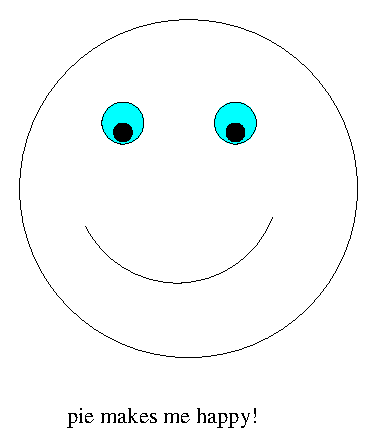
\includegraphics[width=0.4\textwidth]{fig.eps}
%%    \caption[Happy Face: figure example.]{\label{fig:happy} This is a figure of
%%      a happy face with a \texttt{psfrag} replacement.  The original figure
%%      (drawn in xfig and exported to a .eps file) has the text ``pie makes me
%%      happy!''.  The \texttt{psfrag} package replaces this with ``$\pi$ makes me
%%      happy!''.  Note: the Makefile compiles the sample using pdf\LaTeX\ which
%%      cannot use \texttt{psfrag} directly.  For some options that work with
%%      pdf\LaTeX, please see this discussion:
%%      \url{http://tex.stackexchange.com/questions/11839}.  For the caption, we
%%      have used the optional argument for the caption command so that only a
%%      short version of this caption occurs in the list of figures.}
%%  \end{center}
%%\end{figure}
%%\afterpage{\clearpage}
%%Here is an example of a figure environment.
%%Perhaps I should say that the example of a figure can be seen in
%%Figure~\ref{fig:happy}.  Figure placement can be tricky with \LaTeX\
%%because figures and tables are treated as ``floats'': text can flow
%%around them, but if there is not enough space, they will appear later.
%%To prevent figures from going too far, the
%%\verb|\afterpage{\clearpage}| command can be used.  This makes sure
%%that the figure are typeset at the end of the page (possibly appear on
%%their own on the following pages) and before any subsequent text.
%%
%%The \verb|\clearpage| forces a page break so that the figure can be
%%placed, but without the the \verb|\afterpage{}| command, the page
%%would be broken too early (at the \verb|\clearpage| statement).  The
%%\verb|\afterpage{}| command tells \LaTeX{} to issue the command after
%%the present page has been rendered.
%%
%%\section{Tables}
%%We have already included one table:~\ref{tab:Table1}.  Another table
%%is plopped right here.
%%\begin{table}[ht]
%%  \begin{center}
%%    \begin{tabular}{|l||l|l||l|l|}
%%      \hline
%%      &\multicolumn{2}{l|}{Singular}&\multicolumn{2}{l|}{Plural}\\
%%      \cline{2-5}
%%       &English&\textbf{Gaeilge}&English&\textbf{Gaeilge}\\
%%      \hline\hline
%%      1st Person&at me&\textbf{agam}&at us&\textbf{againn}\\
%%      2nd Person&at you&\textbf{agat}&at you&\textbf{agaibh}\\
%%      3rd Person&at him&\textbf{aige}&at them&\textbf{acu}\\
%%       &at her&\textbf{aici}& & \\
%%      \hline
%%    \end{tabular}
%%    \caption{
%%      \label{tab:Table2}
%%      Another table.}
%%  \end{center}
%%\end{table}
%%Well, actually, as with Figures, tables do not
%%necessarily appear right ``here'' because tables are also ``floats''.
%%\LaTeX{} puts them where it can.  Because of this, one should refer to
%%floats by their labels rather than by their location.  This example is
%%demonstrated by Table~\ref{tab:Table2}.  This one is pretty close,
%%however.  (Note: you should generally not put tables or figures in the
%%middle of a paragraph.  This example is for demonstration purposes
%%only.)
%%
%%Another useful package is \verb|\usepackage{longtable}| which provides
%%the \texttt{longtable} environment.  This is nice because it allows
%%tables to span multiple pages.  Table~\ref{tab:longtable} has been
%%formatted this way.
%%\begin{center}
%%  \begin{longtable}{|l|l|l|}
%%    \caption{\label{tab:longtable}Feasible triples for
%%      highly variable Grid}\\
%%
%%    \hline \multicolumn{1}{|c|}{\textbf{Time (s)}} &
%%    \multicolumn{1}{c|}{\textbf{Triple chosen}} &
%%    \multicolumn{1}{c|}{\textbf{Other feasible triples}} \\ \hline
%%    \endfirsthead
%%
%%    \multicolumn{3}{c}%
%%    {{\bfseries \tablename\ \thetable{} -- continued from previous page}} \\
%%    \hline \multicolumn{1}{|c|}{\textbf{Time (s)}} &
%%    \multicolumn{1}{c|}{\textbf{Triple chosen}} &
%%    \multicolumn{1}{c|}{\textbf{Other feasible triples}} \\ \hline
%%    \endhead
%%
%%    \hline \multicolumn{3}{|r|}{{Continued on next page}} \\ \hline
%%    \endfoot
%%
%%    \hline \hline
%%    \endlastfoot
%%
%%    0 & (1, 11, 13725) & (1, 12, 10980), (1, 13, 8235), (2, 2, 0), (3, 1, 0) \\
%%    274 & (1, 12, 10980) & (1, 13, 8235), (2, 2, 0), (2, 3, 0), (3, 1, 0) \\
%%    5490 & (1, 12, 13725) & (2, 2, 2745), (2, 3, 0), (3, 1, 0) \\
%%    8235 & (1, 12, 16470) & (1, 13, 13725), (2, 2, 2745), (2, 3, 0), (3, 1, 0) \\
%%    10980 & (1, 12, 16470) & (1, 13, 13725), (2, 2, 2745), (2, 3, 0), (3, 1, 0) \\
%%    13725 & (1, 12, 16470) & (1, 13, 13725), (2, 2, 2745), (2, 3, 0), (3, 1, 0) \\
%%    16470 & (1, 13, 16470) & (2, 2, 2745), (2, 3, 0), (3, 1, 0) \\
%%    19215 & (1, 12, 16470) & (1, 13, 13725), (2, 2, 2745), (2, 3, 0), (3, 1, 0) \\
%%    21960 & (1, 12, 16470) & (1, 13, 13725), (2, 2, 2745), (2, 3, 0), (3, 1, 0) \\
%%    24705 & (1, 12, 16470) & (1, 13, 13725), (2, 2, 2745), (2, 3, 0), (3, 1, 0) \\
%%    27450 & (1, 12, 16470) & (1, 13, 13725), (2, 2, 2745), (2, 3, 0), (3, 1, 0) \\
%%    30195 & (2, 2, 2745) & (2, 3, 0), (3, 1, 0) \\
%%    32940 & (1, 13, 16470) & (2, 2, 2745), (2, 3, 0), (3, 1, 0) \\
%%    35685 & (1, 13, 13725) & (2, 2, 2745), (2, 3, 0), (3, 1, 0) \\
%%    38430 & (1, 13, 10980) & (2, 2, 2745), (2, 3, 0), (3, 1, 0) \\
%%    41175 & (1, 12, 13725) & (1, 13, 10980), (2, 2, 2745), (2, 3, 0), (3, 1, 0) \\
%%    43920 & (1, 13, 10980) & (2, 2, 2745), (2, 3, 0), (3, 1, 0) \\
%%    46665 & (2, 2, 2745) & (2, 3, 0), (3, 1, 0) \\
%%    49410 & (2, 2, 2745) & (2, 3, 0), (3, 1, 0) \\
%%    52155 & (1, 12, 16470) & (1, 13, 13725), (2, 2, 2745), (2, 3, 0), (3, 1, 0) \\
%%    54900 & (1, 13, 13725) & (2, 2, 2745), (2, 3, 0), (3, 1, 0) \\
%%    57645 & (1, 13, 13725) & (2, 2, 2745), (2, 3, 0), (3, 1, 0) \\
%%    60390 & (1, 12, 13725) & (2, 2, 2745), (2, 3, 0), (3, 1, 0) \\
%%    63135 & (1, 13, 16470) & (2, 2, 2745), (2, 3, 0), (3, 1, 0) \\
%%    65880 & (1, 13, 16470) & (2, 2, 2745), (2, 3, 0), (3, 1, 0) \\
%%    68625 & (2, 2, 2745) & (2, 3, 0), (3, 1, 0) \\
%%    71370 & (1, 13, 13725) & (2, 2, 2745), (2, 3, 0), (3, 1, 0) \\
%%    74115 & (1, 12, 13725) & (2, 2, 2745), (2, 3, 0), (3, 1, 0) \\
%%    76860 & (1, 13, 13725) & (2, 2, 2745), (2, 3, 0), (3, 1, 0) \\
%%    79605 & (1, 13, 13725) & (2, 2, 2745), (2, 3, 0), (3, 1, 0) \\
%%    82350 & (1, 12, 13725) & (2, 2, 2745), (2, 3, 0), (3, 1, 0) \\
%%    85095 & (1, 12, 13725) & (1, 13, 10980), (2, 2, 2745), (2, 3, 0), (3, 1, 0) \\
%%    87840 & (1, 13, 16470) & (2, 2, 2745), (2, 3, 0), (3, 1, 0) \\
%%    90585 & (1, 13, 16470) & (2, 2, 2745), (2, 3, 0), (3, 1, 0) \\
%%    93330 & (1, 13, 13725) & (2, 2, 2745), (2, 3, 0), (3, 1, 0) \\
%%    96075 & (1, 13, 16470) & (2, 2, 2745), (2, 3, 0), (3, 1, 0) \\
%%    98820 & (1, 13, 16470) & (2, 2, 2745), (2, 3, 0), (3, 1, 0) \\
%%    101565 & (1, 13, 13725) & (2, 2, 2745), (2, 3, 0), (3, 1, 0) \\
%%    104310 & (1, 13, 16470) & (2, 2, 2745), (2, 3, 0), (3, 1, 0) \\
%%    107055 & (1, 13, 13725) & (2, 2, 2745), (2, 3, 0), (3, 1, 0) \\
%%    109800 & (1, 13, 13725) & (2, 2, 2745), (2, 3, 0), (3, 1, 0) \\
%%    112545 & (1, 12, 16470) & (1, 13, 13725), (2, 2, 2745), (2, 3, 0), (3, 1, 0) \\
%%    115290 & (1, 13, 16470) & (2, 2, 2745), (2, 3, 0), (3, 1, 0) \\
%%    118035 & (1, 13, 13725) & (2, 2, 2745), (2, 3, 0), (3, 1, 0) \\
%%    120780 & (1, 13, 16470) & (2, 2, 2745), (2, 3, 0), (3, 1, 0) \\
%%    123525 & (1, 13, 13725) & (2, 2, 2745), (2, 3, 0), (3, 1, 0) \\
%%    126270 & (1, 12, 16470) & (1, 13, 13725), (2, 2, 2745), (2, 3, 0), (3, 1, 0) \\
%%    129015 & (2, 2, 2745) & (2, 3, 0), (3, 1, 0) \\
%%    131760 & (2, 2, 2745) & (2, 3, 0), (3, 1, 0) \\
%%    134505 & (1, 13, 16470) & (2, 2, 2745), (2, 3, 0), (3, 1, 0) \\
%%    137250 & (1, 13, 13725) & (2, 2, 2745), (2, 3, 0), (3, 1, 0) \\
%%    139995 & (2, 2, 2745) & (2, 3, 0), (3, 1, 0) \\
%%    142740 & (2, 2, 2745) & (2, 3, 0), (3, 1, 0) \\
%%    145485 & (1, 12, 16470) & (1, 13, 13725), (2, 2, 2745), (2, 3, 0), (3, 1, 0) \\
%%    148230 & (2, 2, 2745) & (2, 3, 0), (3, 1, 0) \\
%%    150975 & (1, 13, 16470) & (2, 2, 2745), (2, 3, 0), (3, 1, 0) \\
%%    153720 & (1, 12, 13725) & (2, 2, 2745), (2, 3, 0), (3, 1, 0) \\
%%    156465 & (1, 13, 13725) & (2, 2, 2745), (2, 3, 0), (3, 1, 0) \\
%%    159210 & (1, 13, 13725) & (2, 2, 2745), (2, 3, 0), (3, 1, 0) \\
%%    161955 & (1, 13, 16470) & (2, 2, 2745), (2, 3, 0), (3, 1, 0) \\
%%    164700 & (1, 13, 13725) & (2, 2, 2745), (2, 3, 0), (3, 1, 0) \\
%%\end{longtable}
%%\end{center}
%%
%%\subsection*{An Unnumbered Subsection}
%%Note that if you use subsections or further divisions under an
%%unnumbered section, then you should make them unnumbered as well
%%otherwise you will end up with zeros in the section numbering.
%%
%%\chapter{Landscape Mode}
%%The landscape mode allows you to rotate a page through 90 degrees.  It
%%is generally not a good idea to make the chapter heading landscape,
%%but it can be useful for long tables etc.
%%
%%\begin{landscape}
%%  This text should appear rotated, allowing for formatting of very
%%  wide tables etc.  Note that this might only work after you convert
%%  the \texttt{dvi} file to a postscript (\texttt{ps}) or \texttt{pdf}
%%  file using \texttt{dvips} or \texttt{dvipdf} etc.  This feature is
%%  provided by the \verb|lscape| and the \verb|pdflscape| packages.
%%  The latter is preferred if it works as it also rotates the pages in
%%  the pdf file for easier viewing.
%%\end{landscape}

%% This file is setup to use a bibtex file sample.bib and uses the
%% plain style.  Other styles may be used depending on the conventions
%% of your field of study.
%%
%%% Note: the bibliography must come before the appendices.
\bibliographystyle{plain}
\bibliography{sample}

%% Use this to reset the appendix counter.  Note that the FoGS
%% requires that the word ``Appendices'' appear in the table of
%% contents either before each appendix lable or as a division
%% denoting the start of the appendices.  We take the latter option
%% here.  This is ensured by making the \texttt{appendicestoc} option
%% a default option to the UBC thesis class.

%%% If you only have one appendix, please uncomment the following line.
% \renewcommand{\appendicesname}{Appendix}
\appendix
\chapter{First Appendix}
Here you can have your appendices.  Note that if you only have a
single appendix, you should issue
\verb|\renewcommand{\appendicesname}{Appendix}| before calling
\verb|\appendix| to display the singular ``Appendix'' rather than the
default plural ``Appendices''.

\chapter{Second Appendix}
Here is the second appendix.

%% This changes the headings and chapter titles (no numbers for
%% example).
\backmatter

%% Indices come here if you have them.

%%\chapter*{Additional Information}
%%This chapter shows you how to include additional information in your
%%thesis, the removal of which will not affect the submission.  Such
%%material should be removed before the thesis is actually submitted.
%%
%%First, the chapter is unnumbered and not included in the Table of
%%Contents.  Second, it is the last section of the thesis, so its
%%removal will not alter any of the page numbering etc. for the previous
%%sections.  Do not include any floats, however, as these will appear in
%%the initial lists.
%%
%%The \texttt{ubcthesis} \LaTeX{} class has been designed to aid you in
%%producing a thesis that conforms to the requirements of The
%%University of British Columbia Faculty of Graduate Studies (FoGS).
%%
%%Proper use of this class and sample is highly recommended---and should
%%produce a well formatted document that meets the FoGS requirement.
%%Notwithstanding, complex theses may require additional formatting that
%%may conflict with some of the requirements.  We therefore \emph{highly
%%  recommend} that you consult one of the FoGS staff for assistance and
%%an assessment of potential problems \emph{before} starting final
%%draft.
%%
%%While we have attemped to address most of the thesis formatting
%%requirements in these files, they do not constitute an official set of
%%thesis requirements.  The official requirements are available at the
%%following section of the FoGS web site:
%%\begin{center}
%%  \begin{tabular}{|l|}
%%    \hline
%%    \url{http://www.grad.ubc.ca/current-students/dissertation-thesis-preparation}\\
%%    \hline
%%  \end{tabular}
%%\end{center}
%%We recommend that you review these instructions carefully.

\end{document}
\endinput
%%
%% End of file `ubcsample.tex'.
